\documentclass[11pt,a4paper]{article}
\usepackage[margin=22mm]{geometry}
\usepackage[T1]{fontenc}
\usepackage{lmodern,array,tabularx,booktabs,graphicx,hyperref,xcolor}
\setlength{\parindent}{0pt}\setlength{\parskip}{6pt}

\begin{document}

\begin{center}\Large\textbf{23CSE455 Design Patterns}\\[4pt]\LARGE Case Study Report\end{center}

\textbf{Team:} B12\par
\textbf{Case study:} Design Pattern Identification and Evolution in a NestJS-Based Parking Management Application\par
\textbf{Application:} Smart Parking Reservation System\par
\textbf{Date:} 2026-10-10\par
\textbf{Submission repository:} \href{https://github.com/aswathymohan-amrita/23CSE455_DP_CaseStudy}{23CSE455\_DP\_CaseStudy}\par

\textbf{Students}\par
\begin{tabularx}{\linewidth}{@{}llX@{}}\toprule
Roll number & Student name & Batch\\\midrule
AM.SC.U4CSE23349 & Samanthula Eswar & CSE\\
AM.SC.U4CSE23210 & Bantupalli Harsha Vardhan & CSE\\
AM.SC.U4CSE23344 & Rayudu Vamsi Krishna & CSE\\
AM.SC.U4CSE23350 & Sammeta Pavan & CSE\\\bottomrule
\end{tabularx}

\begin{abstract}
This report studies the design patterns present in the \emph{Smart Parking
Reservation System}, a NestJS/TypeORM backend with a Next.js/React frontend,
inspected at baseline commit \texttt{940daee}. Part~1 reports a baseline
candidate set of four confirmed pattern categories comprising seven recorded
instances: the Strategy pattern (GoF, behavioural; 1 instance) and three
architectural patterns --- Repository (4 instances), Dependency Injection /
Inversion of Control (1 instance) and Layered Architecture (1 instance).
Part~2 implements three evolution changes on top of the baseline --- dynamic
slot allocation (a second Strategy instance), EV charging (introducing the
\textbf{State} pattern) and real-time occupancy monitoring (introducing the
\textbf{Observer} pattern) --- each captured as a sequential diff and covered by
passing tests. Part~3 compares all six confirmed pattern types ---
\textbf{Strategy}, \textbf{State}, \textbf{Observer}, \textbf{Repository},
\textbf{Dependency Injection} and \textbf{Layered Architecture} --- across
JavaScript, Python, Java and C++ on lines of code, cyclomatic complexity and
process runtime.
\end{abstract}

\noindent\textbf{Evidence policy.}
Every pattern claim in this report is supported by actual source evidence:
verifiable inspected file paths, code excerpts, and source locations.
LLM-generated assertions alone are insufficient and are not accepted as evidence
for any pattern, pattern count, metric, or test result.

\section{Application and Architecture}
The case study inspects the \emph{Smart Parking Reservation System}, a
full-stack application comprising a NestJS backend and a Next.js frontend.
\begin{itemize}
  \item Application: Smart Parking Reservation System (NestJS backend + Next.js
        frontend).
  \item Repository URL:\\
        \url{https://github.com/nuhu78/Smart-Parking-Reservation-System}
  \item Branch: \texttt{main}.
  \item Baseline commit: \texttt{940daeeab52d5a0b101ce0e76813bcfac88e01a1}\\
        (short \texttt{940daee}).
  \item Access date: 2026-10-10.
  \item Backend stack: NestJS~11, TypeScript, TypeORM and PostgreSQL.
  \item Frontend stack: Next.js, React and Zustand.
  \item Modules in scope: parking-slot management, vehicle management,
        reservation, payment, occupancy, EV charging, notifications.
\end{itemize}

\noindent\textbf{Architecture overview.}
The backend is organised into NestJS feature modules --- \texttt{auth},
\texttt{users}, \texttt{parking}, \texttt{slots}, \texttt{reservations},
\texttt{mail} and \texttt{seed} --- arranged in a
controller $\rightarrow$ service $\rightarrow$ repository layering and wired
together through the Nest dependency-injection container. Persistence is
mediated by TypeORM against PostgreSQL. The frontend consumes the REST API and
holds authentication state in a Zustand store.

\begin{figure}[htbp]
  \centering
  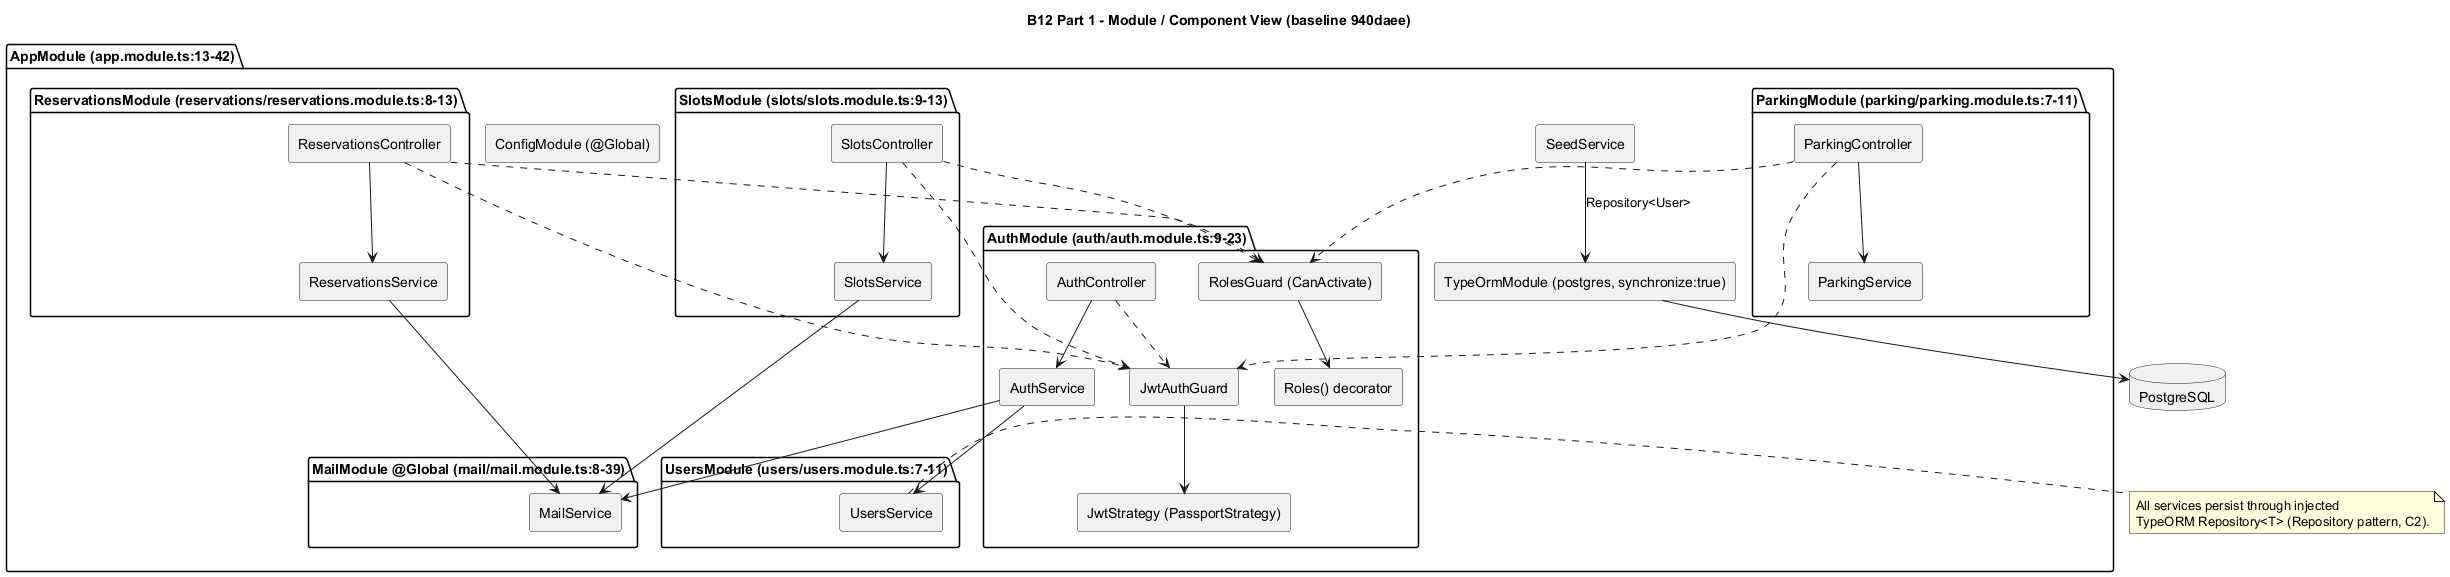
\includegraphics[width=\textwidth]{Part1/diagrams/rendered/module_component.png}
  \caption{Application architecture at baseline commit \texttt{940daee}:
  module/component view of the \texttt{smart-parking-backend} wiring in
  \texttt{app.module.ts} and the feature modules (source:
  \texttt{Part1/diagrams/module\_component.puml}).}
  \label{fig:architecture}
\end{figure}

Figure~\ref{fig:architecture} shows the baseline module wiring; the note on
\texttt{UsersService} records the Repository-pattern instances behind each
service.

\section{Part 1 Pattern Discovery}
Part~1 was performed by direct inspection of the baseline source at commit
\texttt{940daee}. Every pattern claim below cites a real, verified
\texttt{file:line} location recorded in
\path{Part1/evidence/pattern_evidence.md}. A pattern is marked
\emph{confirmed} only when the application source contains the pattern's
participants, responsibilities and relationships; a framework class whose name
merely resembles a pattern is not sufficient. Candidates that could not be
established at application level are recorded as \emph{uncertain} or
\emph{not found} in \path{Part1/evidence/rejected_and_uncertain.md}.

\subsection{Totals at the Baseline}
\begin{sloppypar}
At baseline commit \texttt{940daee}, four pattern categories were confirmed,
comprising \textbf{7 recorded instances} (from
\path{data/pattern_counts.csv}); GoF and architectural patterns are
distinguished explicitly.
\end{sloppypar}

\begin{center}
\begin{tabular}{l l r}
\toprule
Pattern category & Classification & Instances \\
\midrule
Strategy & GoF (behavioural) & 1 \\
Repository & Architectural & 4 \\
Dependency Injection / IoC & Architectural & 1 \\
Layered Architecture & Architectural & 1 \\
\midrule
\textbf{Total} & & \textbf{7} \\
\bottomrule
\end{tabular}
\end{center}

\subsection{Pattern Inventory}
The inventory is the machine-readable content of \texttt{data/patterns.csv}
(7 data rows plus a header) and \path{data/pattern_counts.csv} (4 data rows
plus a header). GoF patterns and architectural patterns are listed separately.

\medskip
\begin{center}
\small
\begin{tabular}{@{}>{\raggedright\arraybackslash}p{0.22\textwidth}
                   >{\raggedright\arraybackslash}p{0.22\textwidth}
                   >{\raggedright\arraybackslash}p{0.50\textwidth}@{}}
\toprule
Pattern & Instance & Source location(s) \\
\midrule
Strategy (GoF, behavioural) & JWT authentication strategy &
\path{auth/strategies/jwt.strategy.ts:7-18};
\path{auth/guards/jwt-auth.guard.ts:1-5};
\path{slots/slots.controller.ts:22-23} \\
\addlinespace
Repository (architectural) & User repository &
\path{users/users.service.ts:9-12} \\
Repository (architectural) & ParkingArea repository &
\path{parking/parking.service.ts:9-11} \\
Repository (architectural) & Slot repository &
\path{slots/slots.service.ts:17-19} \\
Repository (architectural) & Reservation repository &
\path{reservations/reservations.service.ts:15-16} \\
\addlinespace
Dependency Injection / IoC (architectural) & Nest container wiring &
\path{app.module.ts:13-42};
\path{users/users.module.ts:7-11};
\path{slots/slots.controller.ts:24-25};
\path{auth/auth.service.ts:18-22} \\
\addlinespace
Layered Architecture (architectural) & Backend layering &
\path{slots/slots.controller.ts:29-30};
\path{slots/slots.service.ts:29-49};
\path{parking/parking.controller.ts:27-28};
\path{parking/parking.service.ts:14-19} \\
\bottomrule
\end{tabular}
\end{center}

\begin{sloppypar}
\noindent Candidates recorded as \emph{uncertain} (Singleton, Adapter, Template
Method, Factory Method, Chain of Responsibility, Observer, Facade, Data Mapper)
are \textbf{not} counted as confirmed. Rejected candidates (GoF Decorator,
Builder, State, Proxy, Command, Iterator, Abstract Factory, MVC) are documented
in \path{Part1/evidence/rejected_and_uncertain.md}.
\end{sloppypar}

\subsection{One Record for Each Pattern Instance}
Each record gives the pattern category, the instance, the participant roles and
the verified source evidence. The full evidence register is in
\path{Part1/evidence/pattern_evidence.md}.

\paragraph{Strategy (GoF, behavioural) --- JWT authentication strategy.}
\begin{sloppypar}
Concrete strategy: \texttt{JwtStrategy}
(\path{auth/strategies/jwt.strategy.ts:7-18}), which implements the
algorithm-specific \texttt{validate()} step
(\path{auth/strategies/jwt.strategy.ts:22-30}). The strategy is selected
polymorphically by name via \texttt{AuthGuard('jwt')}
(\path{auth/guards/jwt-auth.guard.ts:5}) and used by guarded controllers such
as \path{slots/slots.controller.ts:22-23}. The strategy interface and the
context are supplied by \texttt{passport-jwt}/Passport; the application supplies
the concrete strategy and its registration as a provider
(\path{auth/auth.module.ts:22}). This attribution is stated explicitly rather
than assumed from a class named \texttt{Strategy}.
\end{sloppypar}

\paragraph{Repository (architectural) --- four instances.}
\begin{sloppypar}
User (\path{users/users.service.ts:9-12}), ParkingArea
(\path{parking/parking.service.ts:9-11}), Slot
(\path{slots/slots.service.ts:17-19}) and Reservation
(\path{reservations/reservations.service.ts:15-16}). In each case an
application service depends on an injected typed
\texttt{Repository<\ldots>} (TypeORM) and mediates all persistence for that
entity through it.
\end{sloppypar}

\paragraph{Dependency Injection / Inversion of Control (architectural) --- one
instance.}
\begin{sloppypar}
Dependencies are declared in module \texttt{providers}/\texttt{exports}
metadata and delivered through constructor injection --- for example
\path{app.module.ts:13-42}, \path{users/users.module.ts:7-11},
\path{slots/slots.controller.ts:24-25} and \path{auth/auth.service.ts:18-22}.
\end{sloppypar}

\paragraph{Layered Architecture (architectural) --- one instance.}
\begin{sloppypar}
One-directional call flow
controller $\rightarrow$ service $\rightarrow$ repository, visible across the
\texttt{slots}, \texttt{parking} and \texttt{reservations} modules
(\path{slots/slots.controller.ts:29-30};
\path{slots/slots.service.ts:29-49};
\path{parking/parking.controller.ts:27-28};
\path{parking/parking.service.ts:14-19}).
\end{sloppypar}

\section{Part 2 Evolution and Refactoring}
Three evolution changes were implemented as additive overlays on the baseline
backend. The original application source was \emph{not} modified in place; each
change exists as a set of changed and new source files under
\path{Part2/code/evolved/smart-parking-backend/src/} and a unified diff under
\path{Part2/changes/ChangeN/diff/}. Diffs are sequential: each applies on top of
the previous change's snapshot. Every change was compiled and its tests were run
with Jest 30.2.0 on Node~24.18.0 (results summarised in
\path{test_result/part2_summary.md}; raw logs per change).

\subsection{Change 1 --- Dynamic Slot Allocation (Strategy)}
\textbf{Requirement.} Replace the hard-coded ``first available slot'' choice with
a pluggable allocation policy (first available, nearest to entrance, EV
preferred) selectable per request. \textbf{Pattern.} The existing baseline
Strategy provided by Passport/JWT covers authentication only; this change
introduces an application-level Strategy of its own --- a
\texttt{SlotAllocationStrategy} interface with three concrete strategies and a
\texttt{SlotAllocationContext} that dispatches to the selected policy (default
\path{first-available}, unknown names falling back to it). An additive nullable
\texttt{distanceToEntrance} column was added to the slot entity to support the
nearest-to-entrance policy; existing slot methods are unchanged.
\textbf{Diff.} \path{Change1/diff/change1.diff} --- 10 files, $+249/-1$.
\textbf{Test.} \path{Change1/test_result/jest_change1.txt} --- 1 suite, 8/8 pass.

Figure~\ref{fig:change1} shows the participant structure of the new Strategy.

\begin{figure}[htbp]
  \centering
  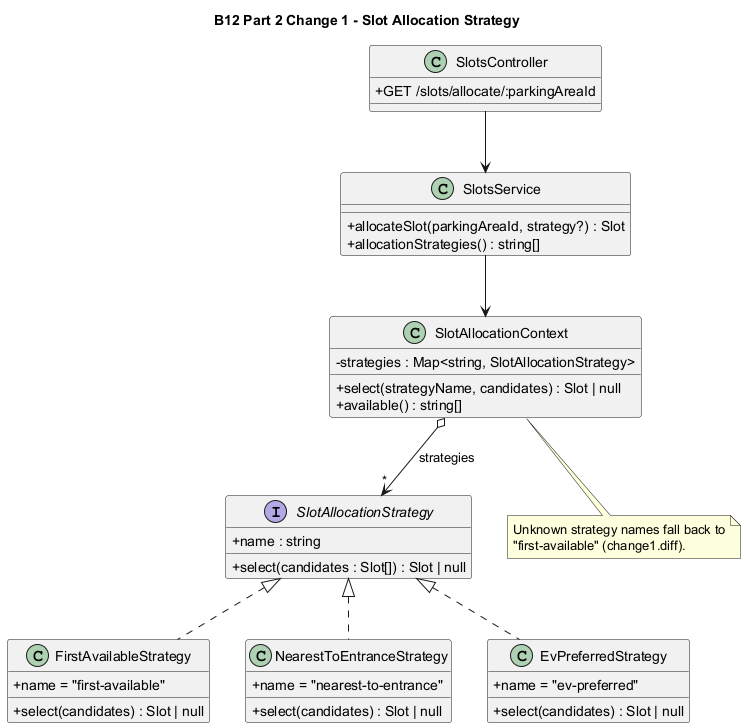
\includegraphics[width=0.8\textwidth]{Part2/diagrams/rendered/change1_strategy.png}
  \caption{Change 1 (Strategy): \texttt{SlotAllocationStrategy} interface, its
  three concrete strategies (\texttt{first-available},
  \texttt{nearest-to-entrance}, \texttt{ev-preferred}) and the
  \texttt{SlotAllocationContext} dispatch (source:
  \texttt{Part2/diagrams/change1\_strategy.puml}).}
  \label{fig:change1}
\end{figure}

\subsection{Change 2 --- EV Charging (State)}
\textbf{Requirement.} Model an EV charging session whose behaviour changes with
its lifecycle state.

\textbf{Pattern.} \begin{sloppypar}This introduces the \textbf{State}
pattern (recorded as rejected/not-found at baseline): a
\texttt{ChargingState} interface with \texttt{Idle}, \texttt{PluggedIn},
\texttt{Charging} and \texttt{Completed} concrete states held by a
\texttt{ChargingSession} context. Legal transitions are \texttt{idle}
$\rightarrow$ \texttt{plugged-in} $\rightarrow$ \texttt{charging}
$\rightarrow$ \texttt{completed} $\rightarrow$ \texttt{idle}, plus an unplug
during charging; illegal operations raise \texttt{BadRequestException}. A
\texttt{ChargingService} / \texttt{ChargingController} expose the session over
REST.\end{sloppypar}

\textbf{Diff.} \path{Change2/diff/change2.diff} --- 8 files, $+302/-1$
(\texttt{app.module.ts} adds \texttt{ChargingModule}).

\textbf{Test.} \path{Change2/test_result/jest_change2.txt} --- 1 suite, 8/8 pass.

Figure~\ref{fig:change2} shows the State-pattern participants and the legal
transitions exercised by the session.

\begin{figure}[htbp]
  \centering
  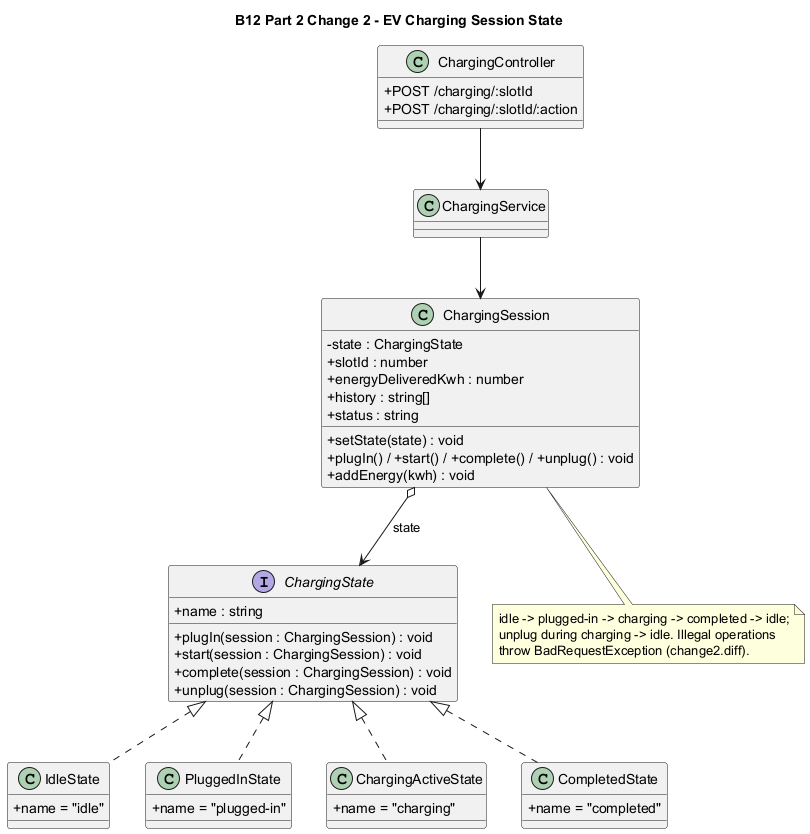
\includegraphics[width=0.75\textwidth]{Part2/diagrams/rendered/change2_state.png}
  \caption{Change 2 (State): \texttt{ChargingState} interface, the four concrete
  states and the \texttt{ChargingSession} context (source:
  \texttt{Part2/diagrams/change2\_state.puml}).}
  \label{fig:change2}
\end{figure}

\subsection{Change 3 --- Real-Time Occupancy Monitoring (Observer)}
\textbf{Requirement.} Notify interested parties whenever a slot's occupancy
changes. \textbf{Pattern.} This introduces the \textbf{Observer} pattern:
\texttt{OccupancyMonitor} is the subject and \texttt{OccupancyObserver} the
observer interface, with a \texttt{LoggingObserver} (appends an event log) and
an \texttt{AvailabilityObserver} (tracks occupied slots and a count). Observers
can be attached and detached at runtime, and are wired in the module. A
controller accepts occupancy updates. \textbf{Diff.}
\path{Change3/diff/change3.diff} --- 8 files, $+177/-1$ (\texttt{app.module.ts}
adds \texttt{OccupancyModule}). \textbf{Test.}
\path{Change3/test_result/jest_change3.txt} --- 1 suite, 5/5 pass.

Figure~\ref{fig:change3} shows the Observer-pattern subject, observers and the
occupancy event flow.

\begin{figure}[htbp]
  \centering
  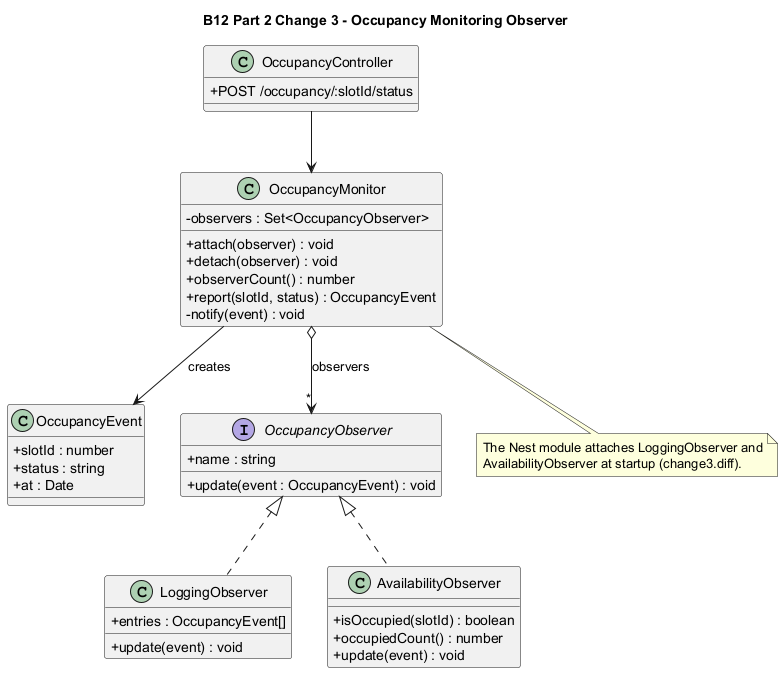
\includegraphics[width=0.8\textwidth]{Part2/diagrams/rendered/change3_observer.png}
  \caption{Change 3 (Observer): \texttt{OccupancyMonitor} subject, the
  \texttt{OccupancyObserver} interface with \texttt{LoggingObserver} and
  \texttt{AvailabilityObserver} (source:
  \texttt{Part2/diagrams/change3\_observer.puml}).}
  \label{fig:change3}
\end{figure}

\subsection{Updated Pattern Counts}
The table below compares the baseline counts with the final post-change counts
(also recorded incrementally in \texttt{data/pattern\_counts.csv}). Change~1 adds
a second Strategy instance (slot allocation) alongside the baseline JWT strategy;
Change~2 introduces State; Change~3 introduces Observer. Repository, DI/IoC and
Layered Architecture remain as at baseline and are reused by the new code.

\begin{center}
\begin{tabular}{l r r}
\toprule
Pattern category & Baseline & After Part 2 \\
\midrule
Strategy & 1 & 2 \\
State & 0 & 1 \\
Observer & 0 & 1 \\
Repository & 4 & 4 \\
Dependency Injection / IoC & 1 & 1 \\
Layered Architecture & 1 & 1 \\
\midrule
\textbf{Total} & \textbf{7} & \textbf{10} \\
\bottomrule
\end{tabular}
\end{center}

\noindent\textbf{Regression status.} Across all three changes the full backend
suite reports 22~passed, 3~failed out of 25. The 21 new Part~2 tests all pass; the
3 failures are pre-existing baseline scaffold defects in
\texttt{auth.controller.spec.ts}, \texttt{auth.service.spec.ts} and
\texttt{mail.service.spec.ts} (Nest cannot resolve their dependencies), which
fail identically on the untouched baseline and are unrelated to Part~2. Evidence:
\path{test_result/part2_jest_full.txt} and
\path{test_result/baseline_preexisting_failures_raw.txt}.

\section{Part 3 Cross-language Comparison}
The six confirmed pattern types central to this case study --- \textbf{Strategy}
(slot allocation), \textbf{State} (EV charging session), \textbf{Observer} (slot
occupancy notification), \textbf{Repository} (user account persistence),
\textbf{Dependency Injection} (notification channel injection) and \textbf{Layered
Architecture} (reservation request handling) --- were each implemented from
scratch in JavaScript, Python, Java and C++, every implementation with a
self-contained test. All 24 suites pass (Strategy 5/5, State 13/13, Observer 8/8,
Repository 8/8, Dependency Injection 6/6 and Layered Architecture 8/8 in every
language). The comparison records lines of code (production snippet only,
excluding blanks, comments and tests), maximum function cyclomatic complexity, and
median whole-process wall time (one warm-up discarded, five runs,
high-resolution timer; compile time excluded). Rules and per-run logs are in
\path{Part3/evidence/} and the snippets under \path{Part3/<Pattern>/<lang>}. This
scope --- one representative instance of \emph{every} confirmed pattern type ---
follows the instruction "for each detected pattern type, implement its small
problem in all four languages"; the decision is recorded in
\path{Part3/Part3_scope_decision_note.md}.

\begin{center}
\small
\begin{tabular}{l l r r r}
\toprule
Pattern & Language & LOC & Max CC & Median ms \\
\midrule
Strategy & JavaScript & 75 & 5 & 80.87 \\
Strategy & Python & 49 & 6 & 112.12 \\
Strategy & Java & 77 & 7 & 185.65 \\
Strategy & C++ & 70 & 8 & 18.98 \\
\midrule
State & JavaScript & 94 & 1 & 73.15 \\
State & Python & 57 & 1 & 67.42 \\
State & Java & 83 & 1 & 173.18 \\
State & C++ & 97 & 2 & 20.83 \\
\midrule
Observer & JavaScript & 56 & 3 & 75.32 \\
Observer & Python & 33 & 3 & 65.18 \\
Observer & Java & 44 & 3 & 159.11 \\
Observer & C++ & 44 & 3 & 15.94 \\
\midrule
Repository & JavaScript & 58 & 2 & 78.93 \\
Repository & Python & 43 & 1 & 104.62 \\
Repository & Java & 56 & 1 & 143.41 \\
Repository & C++ & 46 & 2 & 16.19 \\
\midrule
Dependency Injection & JavaScript & 43 & 1 & 80.49 \\
Dependency Injection & Python & 25 & 1 & 45.41 \\
Dependency Injection & Java & 36 & 1 & 141.08 \\
Dependency Injection & C++ & 34 & 1 & 17.05 \\
\midrule
Layered Architecture & JavaScript & 51 & 2 & 74.70 \\
Layered Architecture & Python & 34 & 3 & 89.70 \\
Layered Architecture & Java & 53 & 3 & 148.05 \\
Layered Architecture & C++ & 48 & 3 & 15.81 \\
\bottomrule
\end{tabular}
\end{center}

Python produces the shortest snippets; Java and C++ are the most verbose; the
statically linked C++ binaries are roughly an order of magnitude faster, while the
timed Java and Python figures are dominated by VM/interpreter startup. Cyclomatic
complexity is low throughout: the State, Dependency Injection and (most)
Repository snippets are branch-free in the garbage-collected languages (CC~1)
because behaviour is delegated to polymorphic or injected collaborators.
Strategy has the highest complexity --- C++ reaches 8 through the null guards its
pointer-returning \texttt{choose()} requires --- while Observer carries a
subscriber loop and a detach guard (CC~3) in every language. All values are
taken directly from \texttt{data/cross\_language.csv}.

\section{LLM Records and Human Verification}
Four LLM artifacts are recorded for this case study: the members' shared ChatGPT
conversations about the assignment, kept as research artifacts only. No LLM was
used to produce the Part~2 or Part~3 code, tests or metrics, and no new prompt was
issued for Part~2 (see \path{Part2/prompts/Part2_prompt.txt}). The full record is
in \texttt{data/llm.csv}; the reference index is
\path{LLM_RESEARCH_REFERENCES.md} and the per-member mapping is in
\path{CONTRIBUTIONS.md}.

\begin{center}
\small
\begin{tabular}{@{}p{0.30\textwidth} p{0.24\textwidth} p{0.38\textwidth}@{}}
\toprule
Member & Conversation topic & Conversation \\
\midrule
Samanthula Eswar (23349) & Pattern analysis (Parts 1--3) & \href{https://chatgpt.com/share/6aca22a9-2844-83ec-8126-e6f81ef8e85e}{share page} \\
Bantupalli Harsha Vardhan (23210) & Pattern discovery report & \href{https://chatgpt.com/share/6acf4ad3-5900-83ee-bd23-a3440efaf33a}{share page} \\
Rayudu Vamsi Krishna (23344) & Pattern discovery report & \href{https://chatgpt.com/share/6acf4a3b-0d60-83ee-af0e-eb5a739699e1?ogimg=plain}{share page} \\
Sammeta Pavan (23350) & Pattern discovery analysis & \href{https://chatgpt.com/share/6acf5448-c740-83e8-b064-e5604a16fb75?ogimg=plain}{share page} \\
\bottomrule
\end{tabular}
\end{center}

The exact model and date are not shown by any share page. None of these
conversations is independently verified as correct; each is treated as a research
artifact only, never as evidence for any pattern, count, metric or test result.
Index: \path{LLM_RESEARCH_REFERENCES.md}; per-member mapping:
\path{CONTRIBUTIONS.md}.

\begin{quote}
LLM outputs are recorded as artifacts only. Every claim derived from an LLM
response must be independently verified against the actual source code before
it may appear anywhere in this report. LLM assertions alone are insufficient.
\end{quote}

\section{Findings, Contributions and References}
\begin{sloppypar}
\textbf{Findings.} (i) At baseline the application confirms four pattern
categories and seven instances (Strategy, four Repository instances, DI/IoC and
Layered Architecture); payment, EV charging and occupancy monitoring are absent
as modules. (ii) The three Part~2 changes each fit an existing architectural
style: Change~1 adds an application Strategy alongside the Passport/JWT Strategy,
Change~2 introduces State, and Change~3 introduces Observer --- the last two
having been recorded as rejected/not-found at baseline. (iii) All 21 new tests
pass; the only suite failures are three pre-existing baseline defects unrelated
to the changes. (iv) In the cross-language study all six confirmed pattern types
were implemented in the four languages; the State, Dependency Injection and most
Repository variants are branch-free in the garbage-collected languages, Python is
the most concise, Java the most verbose, and the native C++ binary is roughly an
order of magnitude faster than the VM/interpreter languages when timing includes
runtime startup.
\end{sloppypar}

\begin{sloppypar}
\noindent\textbf{Contributions.} The following records the team's \emph{declared}
work division; it does not claim independently verified authorship of individual
files (the repository has a single Git author). Members (batch CSE): Samanthula
Eswar (AM.SC.U4CSE23349), Bantupalli Harsha Vardhan (AM.SC.U4CSE23210), Rayudu
Vamsi Krishna (AM.SC.U4CSE23344) and Sammeta Pavan (AM.SC.U4CSE23350).
\end{sloppypar}

\begin{center}
\small
\begin{tabular}{@{}p{0.46\textwidth} p{0.42\textwidth}@{}}
\toprule
Task & Declared responsibility \\
\midrule
Part 1 --- pattern discovery and source-code analysis & Shared by all four members \\
Part 1 --- report, evidence and UML diagrams & Shared by all four members \\
Part 2 --- three evolution scenarios and implementation & Shared by all four members \\
Part 3 --- Java, Python, JavaScript and C++ implementations & Shared by all four members \\
Testing, metrics and CSV validation & Shared by all four members \\
Final report, integration and submission & Eswar leads \\
\bottomrule
\end{tabular}
\end{center}

\begin{sloppypar}
Parts~1--3, testing, metrics and CSV validation were therefore collaborative
efforts of all four members; Eswar led final report preparation, integration and
submission (team declaration). Deliverables produced by the team: runnable
artifacts for Parts~2--3; per-change requirement notes, sequential diffs and raw
test logs; a reproducible cross-language benchmark with raw evidence; and
machine-readable datasets (\texttt{patterns.csv}, \texttt{pattern\_counts.csv},
\texttt{patterns\_evolution.csv}, \texttt{cross\_language.csv}, \texttt{llm.csv}).
The full declaration and the four conversation links are in
\path{CONTRIBUTIONS.md}.
\end{sloppypar}

\noindent\textbf{References.}
\begin{sloppypar}
\begin{itemize}
  \item \texttt{Smart Parking Reservation System} (baseline source; commit
        \texttt{940daee}): \url{https://github.com/nuhu78/Smart-Parking-Reservation-System}
  \item Assignment repository (course): \url{https://github.com/aswathymohan-amrita/23CSE455_DP_CaseStudy}
  \item Recorded LLM research conversations (ChatGPT shared, one per member):
        \url{https://chatgpt.com/share/6aca22a9-2844-83ec-8126-e6f81ef8e85e};
        \url{https://chatgpt.com/share/6acf4ad3-5900-83ee-bd23-a3440efaf33a};
        \url{https://chatgpt.com/share/6acf4a3b-0d60-83ee-af0e-eb5a739699e1?ogimg=plain};
        \url{https://chatgpt.com/share/6acf5448-c740-83e8-b064-e5604a16fb75?ogimg=plain}.
        Per-member mapping in \path{CONTRIBUTIONS.md}.
\end{itemize}
\end{sloppypar}
Formal bibliographic citations (for example the GoF book) are not yet included
in this section.

\section{Limitations}
\begin{itemize}
  \item This is a baseline source-code study. It does not claim that any missing
        feature has been, or will be, implemented.
  \item At the \textbf{baseline} the following were \textbf{not found} in the
        inspected source: payment, EV charging, occupancy monitoring as a module,
        and a dedicated vehicle-management module. Vehicle-related data exists
        only as fields on the \texttt{User} and \texttt{Reservation} entities. EV
        charging and occupancy monitoring were \emph{added} by the Part~2 overlay
        and were not present in the original application.
  \item Framework- and library-provided behaviour (for example NestJS providers,
        TypeORM repositories, Passport strategies and mailer adapters) must not
        automatically be counted as an application-level GoF pattern.
  \item The first Strategy instance relies on the Passport/JWT strategy
        integration supplied by the application (\texttt{JwtStrategy}) within the
        context provided by Passport; the second (slot allocation) is entirely
        application-level and was introduced in Part~2. Both attributions are
        valid only within the evidence and scope stated in this report.
  \item Pattern counts follow the counting rule documented in the Part 1 report
        and cover both the baseline commit and the Part~2 overlay snapshots; they
        are not performance or quality metrics.
  \item The baseline backend has no committed \texttt{node\_modules} and its
        \texttt{package-lock.json} is out of sync, so \texttt{npm ci} fails; the
        Part~2 tests were therefore run with \texttt{npm install} inside a
        disposable copy of the backend, and the baseline itself was never
        modified.
  \item The Part~2 diffs were produced from sequential snapshots of only the
        added/changed files; they are not full-repository diffs.
\end{itemize}

\section{Team Folder and Datasets}
\begin{sloppypar}
Team folder: \texttt{B12/}
\begin{itemize}
  \item \texttt{data/patterns.csv} --- one row per baseline pattern instance
        (7 data rows plus a header)
  \item \path{data/patterns_evolution.csv} --- per-version pattern evolution
        records (34 data rows plus a header)
  \item \path{data/pattern_counts.csv} --- per-version pattern counts, with
        per-pattern and total rows (27 data rows plus a header)
  \item \path{data/cross_language.csv} --- cross-language comparison records
        (24 data rows plus a header)
  \item \texttt{data/llm.csv} --- LLM prompt/input/output/verification records
        (4 data rows plus a header)
  \item \path{CONTRIBUTIONS.md} --- declared work division and the shared
        ChatGPT conversations
  \item \texttt{Part1/}, \texttt{Part2/}, \texttt{Part3/} --- per-part reports,
        code, evidence, diagrams, prompts and LLM artifacts
  \item \path{test_result/} --- raw Jest logs and the Part~2 summary
        (\path{part2_summary.md}, \path{part2_jest_full.txt},
        \path{baseline_preexisting_failures_raw.txt})
\end{itemize}

\noindent\texttt{patterns.csv} (7 records) and \path{patterns_evolution.csv}
(7 baseline records plus 27 post-change records) hold the Part~1 and Part~2
results; \path{pattern_counts.csv} (6 baseline records plus 21 post-change
records, per-pattern and total rows) summarises the counts per version.
\path{cross_language.csv} holds the 24 Part~3 comparison records and
\texttt{llm.csv} the four honest LLM records, each mapped to a member in
\path{CONTRIBUTIONS.md}.
\end{sloppypar}

\end{document}
